\subsection{Desempeño del Modelo de \textit{machine learning}}

En esta sección se presentan los resultados obtenidos de los diferentes modelos de \textit{machine learning} utilizados para la clasificación de \glspl{url} maliciosas y benignas, así como el análisis de su desempeño basado en las métricas de evaluación empleadas.

\subsubsection*{Modelos Evaluados}
Se evaluaron varios modelos de \textit{machine learning} utilizando la búsqueda de hiperparámetros con \textit{Grid Search} y \textit{Random Search}. Los modelos considerados incluyen:
\begin{itemize}
    \item Árbol de decisión
    \item \textit{Random Forest}
    \item \textit{K-Nearest Neighbors} (KNN)
    \item \textit{XGBoost}
    \item Máquina de Soporte Vectorial (SVM)
    \item \textit{LightGBM}
    \item \textit{Gradient Boosting}
    \item \textit{AdaBoost}
    \item Regresión Logística
\end{itemize}

Además, se utilizaron dos modelos de \textit{stacking} para combinar los resultados de múltiples clasificadores y mejorar el desempeño general.

\subsection{Métricas de Evaluación}
Las métricas de evaluación utilizadas fueron la precisión, el porcentaje de falsos positivos (FP) y el porcentaje de falsos negativos (FN). Estas métricas fueron seleccionadas debido a su importancia en la evaluación de modelos de clasificación, especialmente en el contexto de detección de \textit{phishing} y \glspl{url} maliciosas, donde es crucial minimizar tanto los falsos positivos como los falsos negativos.

\subsubsection*{Resultados de Validación y Prueba}

Las figuras \ref{fig:precision_validacion} y \ref{fig:precision_prueba} muestran la precisión de validación y prueba para los diferentes modelos evaluados. Los modelos \textit{Gradient boost} con \textit{Grid Search} y \textit{Random Search} demostraron ser los más precisos.

\begin{figure}[H]
    \centering
    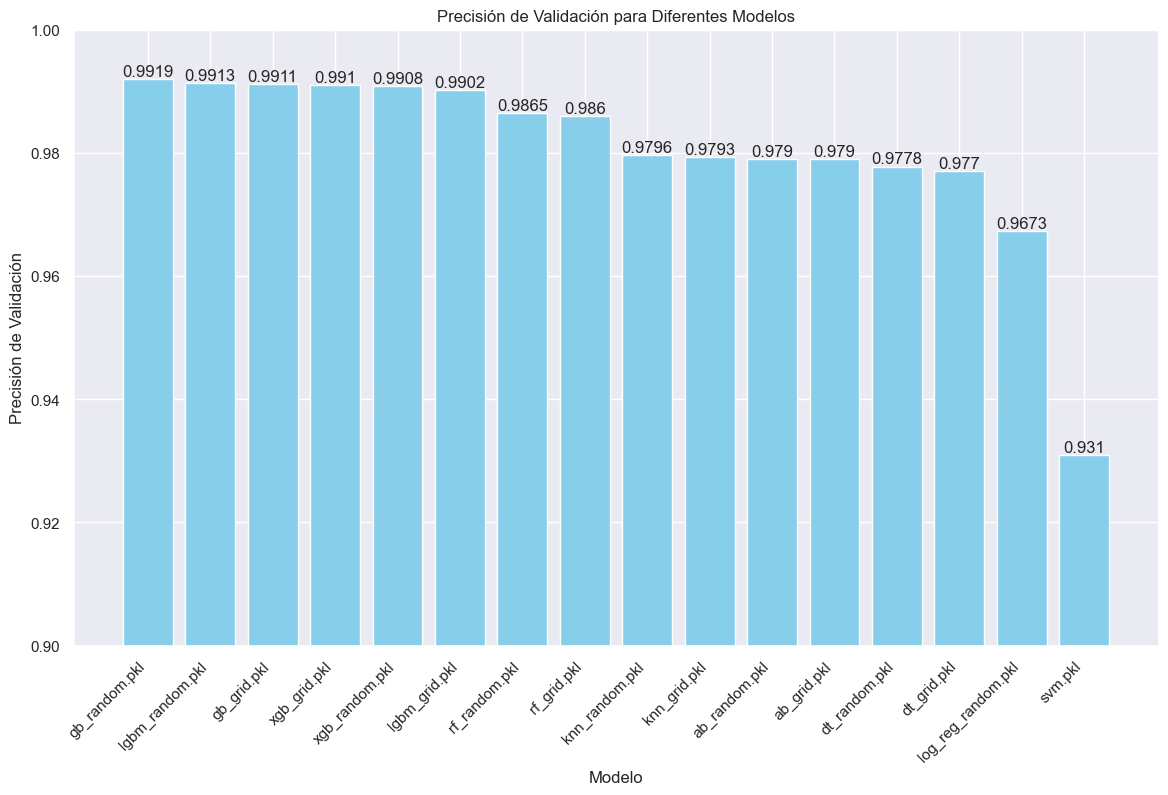
\includegraphics[width=0.8\textwidth]{precisionValidacion.png}
    \caption{Precisión de Validación para Diferentes Modelos}
    \label{fig:precision_validacion}
\end{figure}

\begin{figure}[H]
    \centering
    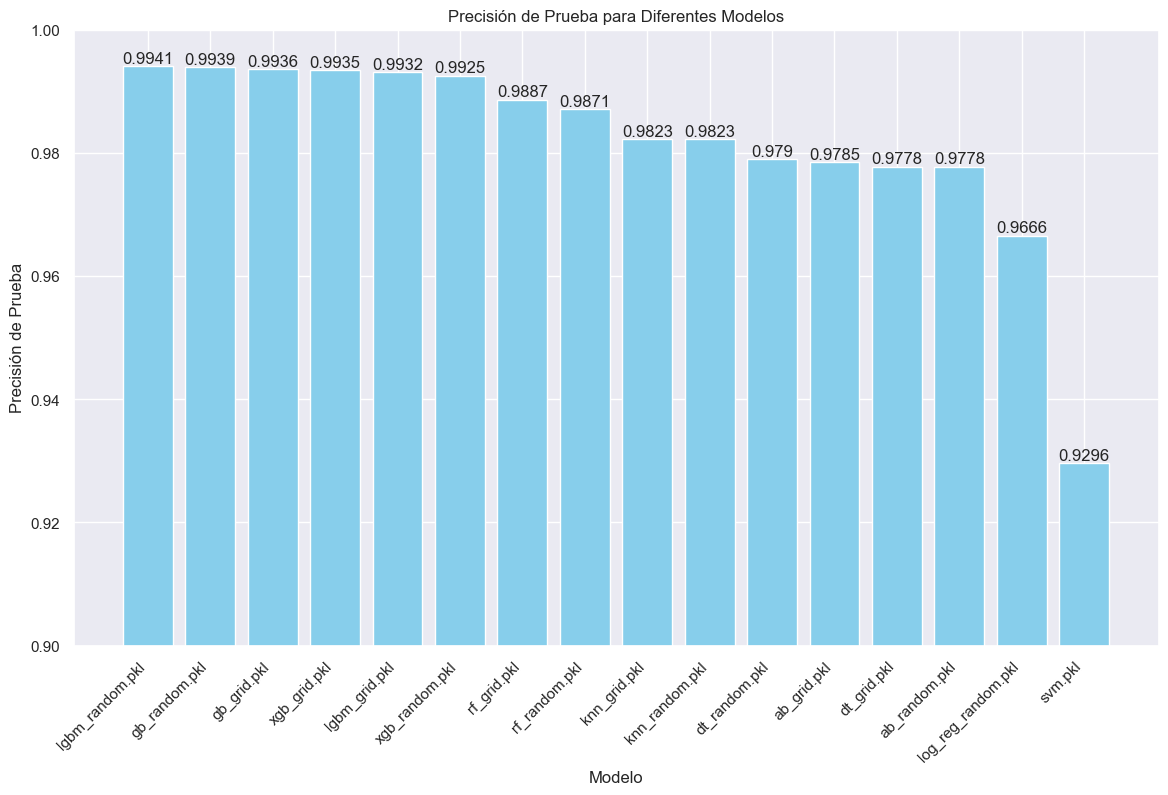
\includegraphics[width=0.8\textwidth]{precisionPrueba.png}
    \caption{Precisión de Prueba para Diferentes Modelos}
    \label{fig:precision_prueba}
\end{figure}

Las figuras \ref{fig:fp_validacion} y \ref{fig:fp_prueba} muestran el porcentaje de falsos positivos en validación y prueba, mientras que las figuras \ref{fig:fn_validacion} y \ref{fig:fn_prueba} muestran el porcentaje de falsos negativos en validación y prueba. Es evidente que el modelo SVM tuvo el mayor porcentaje de falsos positivos y negativos, mientras que los modelos basados en \textit{boosting} presentaron un mejor desempeño en términos de estas métricas.

\begin{figure}[H]
    \centering
    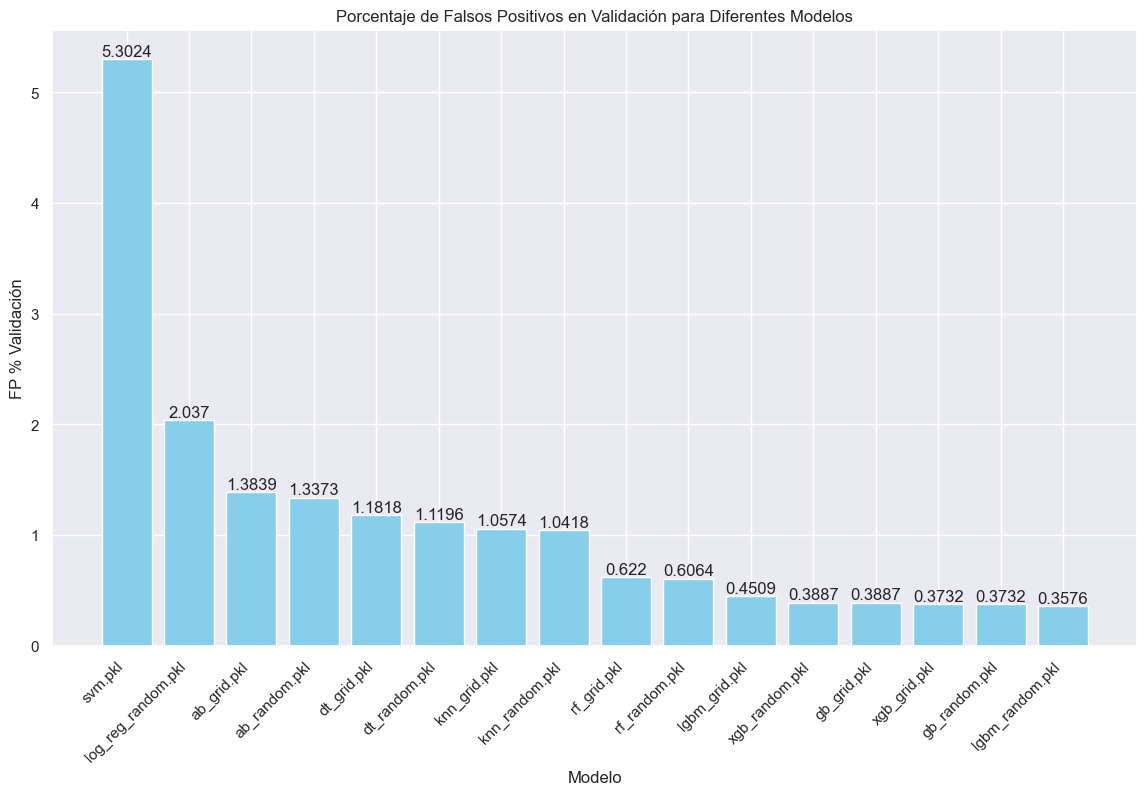
\includegraphics[width=0.8\textwidth]{positivosValidacion.png}
    \caption{Porcentaje de Falsos Positivos en Validación para Diferentes Modelos}
    \label{fig:fp_validacion}
\end{figure}

\begin{figure}[H]
    \centering
    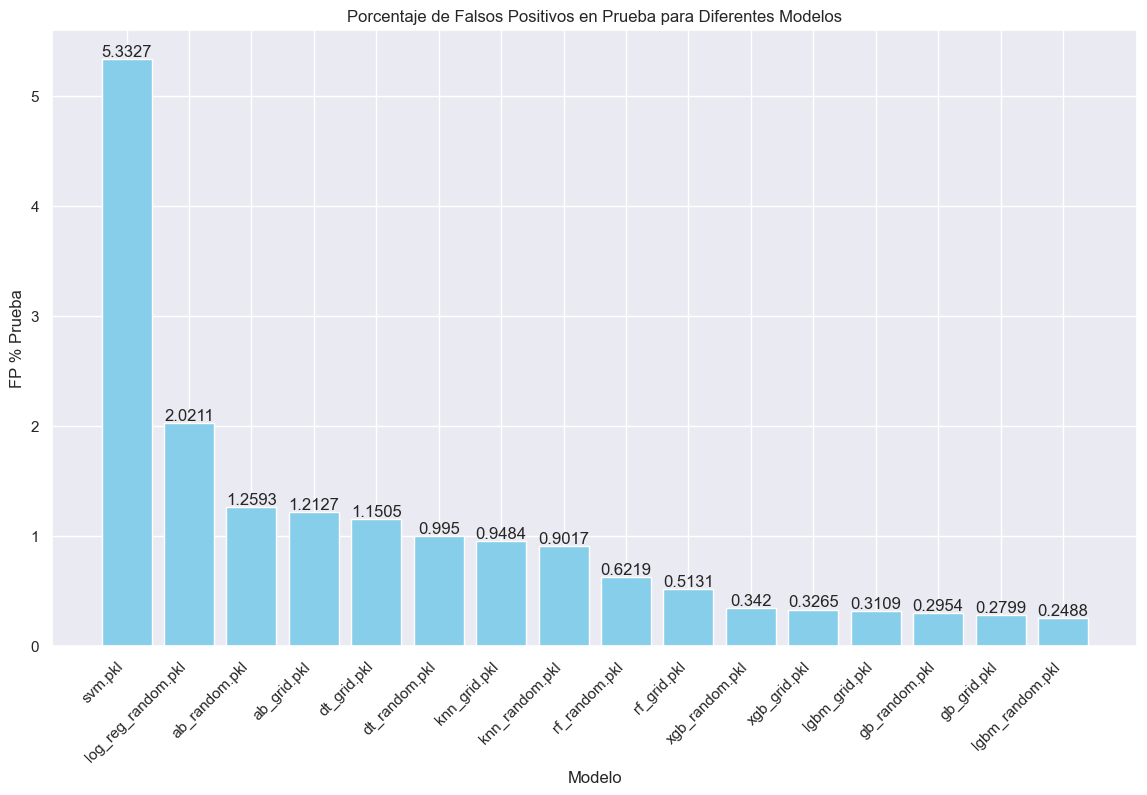
\includegraphics[width=0.8\textwidth]{positivosPrueba.png}
    \caption{Porcentaje de Falsos Positivos en Prueba para Diferentes Modelos}
    \label{fig:fp_prueba}
\end{figure}

\begin{figure}[H]
    \centering
    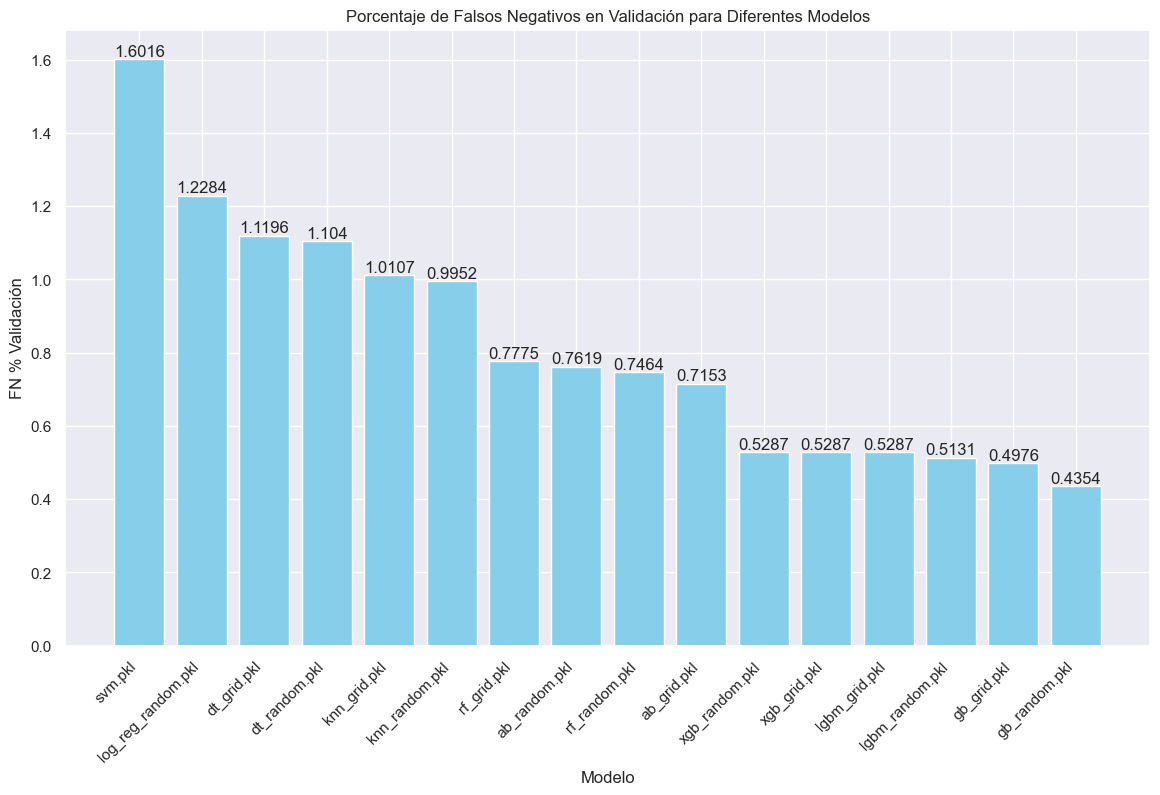
\includegraphics[width=0.8\textwidth]{negativosValidacion.png}
    \caption{Porcentaje de Falsos Negativos en Validación para Diferentes Modelos}
    \label{fig:fn_validacion}
\end{figure}

\begin{figure}[H]
    \centering
    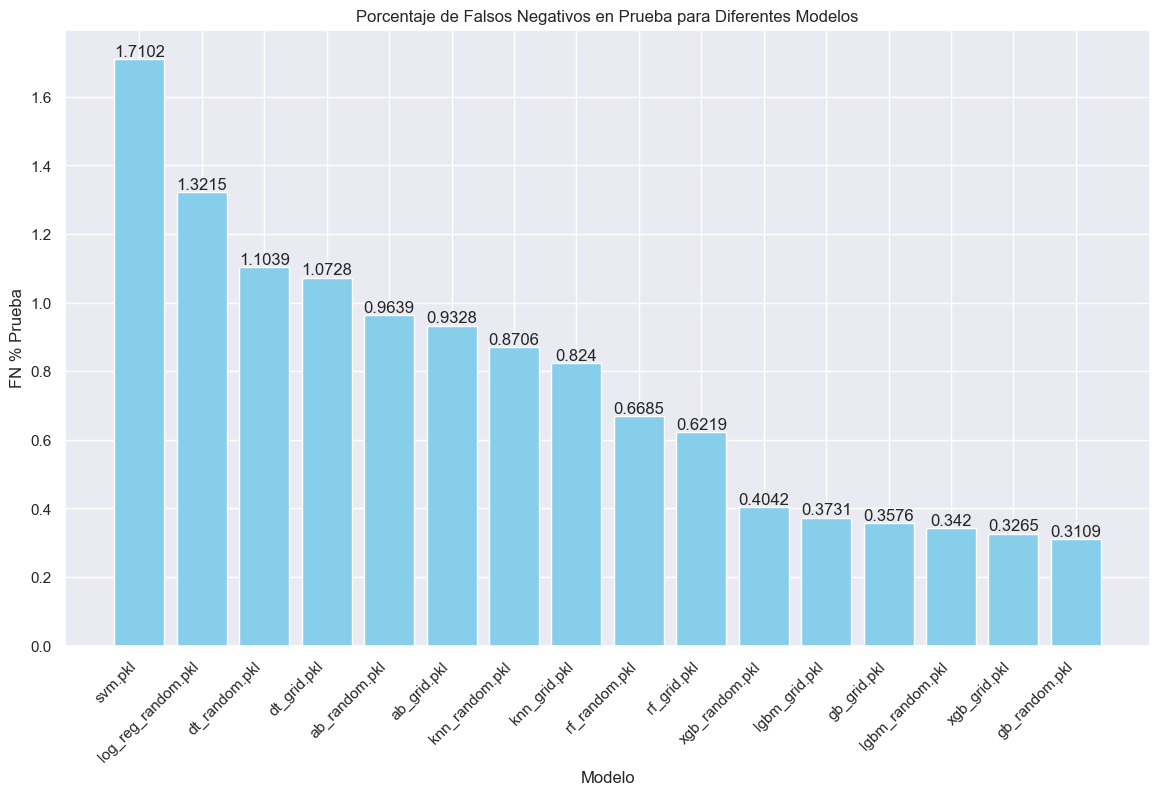
\includegraphics[width=0.8\textwidth]{negativosPrueba.png}
    \caption{Porcentaje de Falsos Negativos en Prueba para Diferentes Modelos}
    \label{fig:fn_prueba}
\end{figure}

\subsubsection*{Modelos de \textit{Stacking}}

El primer modelo de \textit{stacking} combinado mostró una precisión de validación del 98.78\% y una precisión de prueba del 99.00\%, con falsos positivos y falsos negativos inferiores al 0.6\%. El segundo modelo de \textit{stacking}, que utilizó un conjunto diferente de características y clasificadores base, logró una precisión de validación y prueba del 99.17 y 99.28\% respectivamente, con falsos positivos y negativos de apenas 0.40\%.

\begin{table}[H]
    \centering
    \begin{tabular}{lcc}
        \hline
        \textbf{Modelo} & \textbf{Precisión Validación (\%)} & \textbf{Precisión Prueba (\%)} \\
        \hline
        \textit{Stacking 1} & 98.78 & 99.00 \\
        \textit{Stacking 2} & 99.17 & 99.28 \\
        \hline
    \end{tabular}
    \caption{Resultados de Precisión para los Modelos de \textit{Stacking}}
    \label{tab:stacking_results}
\end{table}

El alto desempeño de los modelos de \textit{stacking} destaca su capacidad para combinar las fortalezas de múltiples clasificadores, resultando en un sistema más robusto y preciso para la detección de \glspl{url} maliciosas.


A continuación, se presenta una tabla comparativa de los modelos ordenados por su precisión en el conjunto de prueba:

\begin{table}[H]
    \centering
    \begin{tabular}{lccc}
        \hline
        \textbf{Modelo} & \textbf{Precisión Prueba (\%)} & \textbf{FP Prueba (\%)} & \textbf{FN Prueba (\%)} \\
        \hline
        \textit{Stacking 2} & 99.28 & 0.40 & 0.31 \\
        \textit{Stacking 1} & 99.00 & 0.42 & 0.58 \\
        \textit{xgb\_grid} & 98.94 & 0.46 & 0.6 \\
        \textit{xgb\_random} & 98.83 & 0.50 & 0.66 \\
        \textit{gb\_random} & 99.04 & 0.46 & 0.50 \\
        \textit{gb\_grid} & 98.92 & 0.46 & 0.62 \\
        \textit{log\_reg\_random} & 96.89 & 1.72 & 1.39 \\
        \textit{rf\_grid} & 98.86 & 0.51 & 0.62 \\
        \textit{rf\_random} & 98.70 & 0.62 & 0.67 \\
        \textit{lgbm\_random} & 98.96 & 0.46 & 0.58 \\
        \textit{lgbm\_grid} & 98.88 & 0.52 & 0.60 \\
        \textit{dt\_grid} & 97.77 & 1.15 & 1.07 \\ 
        \textit{dt\_random} & 97.90 & 1.00 & 1.10 \\ 
        \textit{knn\_random} & 97.22 & 1.29 & 1.49 \\
        \textit{knn\_grid} & 97.22 & 1.33 & 1.45 \\
        \textit{ab\_grid} & 98.09 & 1.04 & 0.87 \\
        \textit{ab\_random} & 98.00 & 1.16 & 0.83 \\
        \textit{svm} &  93.01& 5.22 & 1.76 \\
        \hline
    \end{tabular}
    \caption{Comparación de Modelos Ordenados por Precisión en Prueba}
    \label{tab:model_comparison}
\end{table}